\chapter{Introduction}
\label{chap:intro}

\section{Motivation}


Linear least-squares (\stsc{LS}) regression is, without doubt, the workhorse of
data analysis in social sciences, economics and related fields. The reasons for
the popularity of \stsc{LS} regression are obvious. The procedure convinces by
its formal and practical simplicity. \stsc{LS} regression is easy to implement
from a technical point of view and its results, the estimated regression
coefficients, are easy to interpret. Furthermore, \stsc{LS} regression is easy
to teach because its math is relatively simple and is didactically convenient
because \stsc{LS} solutions for small datasets can easily be computed manually
for purpose of exercise and understanding. From a statistical point of view,
\stsc{LS} regression is favorable because it can be shown that under the
assumption of homoscedastic (i.e., equal-variance) and normally distributed
errors the \stsc{LS} estimator is the best (i.e., most efficient) unbiased
estimator (\stsc{BUE}) for the coefficients of a linear regression model. That
is, among all possible unbiased estimators, the \stsc{LS} estimator has the
smallest sampling variance under these conditions.\footnote{Noting the
equivalence between the \stsc{LS} estimator and the arithmetic mean, the
\stsc{BUE} property of the \stsc{LS} estimator is not much of a surprise given
the fact that Carl Friedrich Gauß derived the normal distribution as a
justification for the arithmetic mean. That is, the normal distribution is
\emph{defined} as the distribution under which the \stsc{LS} procedure leads to
the best unbiased estimator for the expected value (for historical background
see \citealp{huber72}).} Also under relaxed assumption, such as non-normal or
heteroscedastic (i.e., non-equal-variance) errors, the \stsc{LS} estimator is
consistent and has, in many cases, good efficiency
properties.\footnote{Although in the later case, the ordinary \stsc{LS} estimate
of the sampling variance is biased and needs to be adjusted by applying
heteroscedasticity-robust variance estimation; see \citealp{white80}.} For
example, in case of homoscedastic non-normal errors, the \stsc{LS} estimator is
the beast linear unbiased estimator (\stsc{BLUE}), that is, has the smallest
sampling variance among all “linear” unbiased estimators.\footnote{The term
“linear” does not refer to the fact that the coefficients of a linear
regression model are to be estimated. An estimator is said to be \emph{linear}
if it is a linear function of the observations $Y_1,\ldots,Y_n$ of the
dependent variable of the regression model. More precisely,
$\sthat{\boldsymbol\beta}$ is a linear estimator of the regression parameters
vector $\boldsymbol\beta \in {\mathbb R}^p$ if there exists a matrix $\stvec{A}
\in {\mathbb R}^{p \times n}$ such that
$\sthat{\boldsymbol\beta}=\stvec{A}\stvec{Y}$ with
$\stvec{Y}=(Y_1,\ldots,Y_n)^t$.}

The outstanding usefulness of \stsc{LS} regression should not be challenged
here. It is important, however, to realize that \stsc{LS} regression may not
always be the best---or at least not the only---choice for analyzing a given
dataset. The restrictiveness of the conditions under which the \stsc{LS}
estimator is deemed best---homoscedasticity and normality of errors---implies
that situations are possible in which alternative estimators can be valuable.
For example, as mentioned above, if the errors are homoscedastic but
non-normal, the \stsc{LS} estimator may be the best linear unbiased estimator,
but this also means that there can be non-linear estimators that, depending on
the nature of the deviation from normality, substantially outperform the
\stsc{LS} estimator in terms of efficiency.\footnote{The limitation to linear
estimators is not much less restrictive than the limitation to normal errors.}
In particular, in case of distributions with heavy tails, that is, if extreme
values are more frequent than in a normal distribution (an example being the
$t$-distribution with few degrees of freedom), the efficiency of the \stsc{LS}
estimator can quickly become poor. Furthermore, the \stsc{LS} estimator may
yield misleading results if the data are “contaminated” by erroneous
observations or, more generally, by a secondary data-generating process.

\paragraph{Efficiency under alternative error distributions}

Assume, for now, that the data are not contaminated and, more or less, follow a
uniform data-generating process that can be described by a linear regression
model. Why, under such a condition, can a low efficiency of the \stsc{LS}
estimator be a problem? Although the
\stsc{LS} estimator is unbiased, more efficient estimators would be preferable
because the precision of an estimator has a direct effect on the value of the
results. For example, the power of a significance test and, therefore, the
potential of the test to find an existing relation, decisively depends on the
efficiency of the employed estimator.

In the context of error distributions with heavy tails the efficiency argument
can also be motivated as follows. Although the \stsc{LS} estimator is unbiased
on average, there is a good chance for a single sample---and in practice often
only one sample is available---to contain extreme values that bias the
regression results in one or the other direction. Robust regression methods
that are less sensitive to such outliers will typically provide more valid
results in such situations, being closer to the true value of the parameter to
be estimated.

Figure~\ref{fig:outliers-and-fits} shows two examples of data sets that have
been generated according to model
\[
    Y = \beta_0 + \beta_1 X + \epsilon
\]
with $\beta_0 = \beta_1 = 0$ (that is, the “true” regression function is a
horizontal line at $y=0$) and $\epsilon$ following a $t$ (Student) distribution with two
degrees of freedom, that is $\epsilon \sim t_2$. Included as lines are the
estimated regression fits using \stsc{LS} estimation, as well as two robust
estimators (an \stsc{M} estimator and an \stsc{MM} estimator). As is evident,
the \stsc{LS} solution is affected by the outliers and suggests a positive
relation between $X$ and $Y$ in the two examples, whereas the two robust
estimator are relatively stable. Robust methods, so to say, contain a safeguard
against extreme data constellations that can occur at random due to sampling or
a stochastic data-generating process. As a diagnostic by-product, robust
methods inform about whether given data are characterized by an anomalous
constellation or not, because only in the former case the results from
\stsc{LS} and the robust methods will substantially differ.


\begin{figure}[h!]
    \centering
    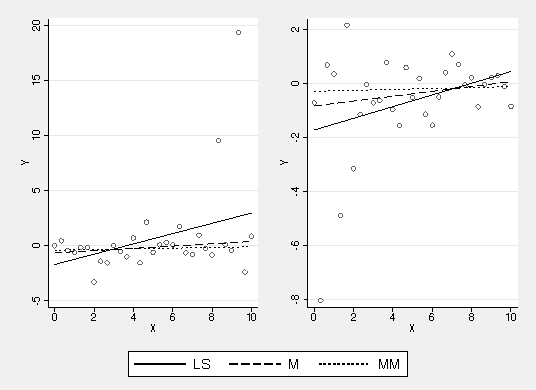
\epsfig{file=eps/2/1}
    \caption{Example scatter plots with outliers and different regression fits}
    \label{fig:outliers-and-fits}
\end{figure}

\paragraph{Bias due to data contamination}

Now assume that the data are “contaminated”, that is, that the majority of data
points follows a well-defined model, but that there are also some observations
that come from a different distribution. For example, while collecting the
data, coding errors could have occurred for some of the observations. In a
study by \citet{jasso85} on the relation between marital duration and coital
frequency there were four observations with a value of 88 for the monthly
coital frequency. Although such values would not be impossible (as argued by
\citealp{jasso85}), the observations were highly suspicious as no other values
of comparable magnitude existed in the data. As argued by \citet{kahnudry86},
the four observations probably were miscoded missing values, whose designated
value was 99. The problem with such miscoded observations is that they can have
strong effects on the results provided by a \stsc{LS} regression. That is,
regression results and the substantive conclusions drawn from them may differ
depending on whether the miscoded observations are kept in the data or not. It
seems important to use methods for data analysis that are able to identify such
problems because, in the words of \citet[18]{anscombe73}, “[w]e are usually
happier about asserting a regression relation if the relation is still apparent
after a few observations (any ones) have been deleted---that is, we are happier
if the regression relation seems to permeate all the observations and does not
derive largely from one or two.”

Conceptually, contamination can be understood as a situation in which the
observed data are the result of a mixture of two or more data-generating
processes. In the case of coding errors there may be a main process of
substantive interest (e.g., the relation between marital duration and coital
frequency), as well as a secondary process (data miscoding by interviewers)
that leads to observations that follow a different distribution and have a
different interpretation. \stsc{LS} regression will not be able to distinguish
the two processes and its results will be valid for neither one of the
processes. If, however, the data are dominated by one of the processes (that
is, if one of the processes is responsible for the bulk of the data) and the
two processes do lead to distinguishable data structures, statistical
procedures to identify the main process are possible. This is where robust
regression comes in. One of the goals of robust regression techniques is to
provide estimates that are resistant against partial contamination of the data.
Robust methods are supposed to correctly identify the primary relation in the
data even if, for example, parts of the data are glaringly erroneous.

An illustrative example comes from astronomy. Figure~\ref{fig:hrdiagram} shows
the Hertzsprung-Russell diagram of star cluster CYG OB1 (see
\citealt[27]{rousseeuw:leroy:1987}). Displayed is the logarithm of the light
intensity of the stars against the logarithm of their effective surface
temperature (using a reversed axis). Furthermore, the graph shows as lines the results of three
different regression estimators, the \stsc{LS} estimator (solid line), a low
breakdown point \stsc{M} estimator (dashed line), and a high breakdown point
\stsc{MM} estimator (dotted line). The results from the \stsc{LS} estimator and
the low breakdown point \stsc{M} estimator are almost identical. They are
strongly influenced by the group of four stars in the upper right corner of the
diagram. In contrast, the high breakdown point \stsc{MM} estimator completely
ignores the four outliers and adequately captures the trend in the main part of
the data. Hence, at least one of the two employed robust estimators
successfully identified the main process (due to the estimator's high breakdown
point; see below).


\begin{figure}[h!]
    \centering
    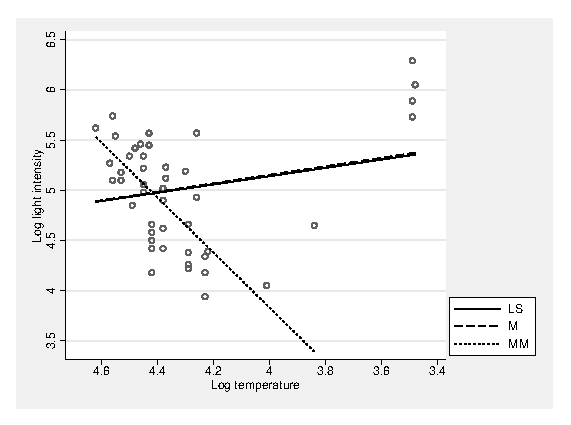
\epsfig{file=eps/2/2}
    \caption{Hertzsprung-Russell diagram of the star cluster CYG OB1 including different regression fits (source: \citealp[27]{rousseeuw:leroy:1987})}
    \label{fig:hrdiagram}
\end{figure}

Again, from a diagnostic perspective, the interesting cases are the ones in
which \stsc{LS} regression and robust estimators lead to differing results.
Substantial differences between robust regression and the \stsc{LS} estimator
indicate that the data cannot be fully descried by a uniform model and that a
part of the observations stands in stark contrast to the main trend in the
data. With the help of the residuals from robust regression, the atypical
observations can be identified and, for example, be subjected to a separate
analysis. In this way, robust regression can contribute to a better
understanding of the data and, potentially, give way to new insights and new
hypotheses. In fact, according to \citet[1]{kruskal60}, the atypical
observations may prove to be the most interesting part of the data: “An
apparently wild (or otherwise anomalous) observation is a signal that says:
`Here is something from which we may learn a lesson, perhaps of a kind not
anticipated beforehand, and perhaps more important than the main object of the
study.'” The four outliers in figure~\ref{fig:hrdiagram}, by the way, are not
errors. The explanation is that there are two different types of stars:
main-sequence stars and giants. That is, conceptually, the observation stem
from two different populations.

\paragraph{Goals and use of robust regression}

To summarize, we can state that robust regression estimators (1) should achieve
good efficiency also in case of non-normal errors and (2) should be resistant
against contamination of the data by outliers. The maximum proportion of
contamination a robust estimator is able to absorb is called the
\emph{breakdown point}.

Both aspects can be formalized with the help of the viewpoint coined by 
\citet{huber64} that observed data follow a mixture distribution
\[
    F_\varepsilon = (1 - \varepsilon) F_{\boldsymbol\theta} + \varepsilon G
\]
where $F_{\boldsymbol\theta}$ is the distribution of interest according to the
supposed model, $G$ is an arbitrary alternative distribution, and $\varepsilon
\in [0,1]$ determines the mixing proportion. For example, in line with the
assumptions of classic linear regression, $F_{\boldsymbol\theta}$ could be a
distribution according to the linear model
\[
    Y = \beta_0 + \beta_1 X + \epsilon
\]
where $X$ has a given distribution and $\epsilon$ is an independent and
identically normally distributed error term. The distribution of the observed
data, however, is contaminated by observations from an unspecified alternative
distribution $G$ and does not fully follow this model. The goal of robust
regression now is to deliver reasonable results for $F_{\boldsymbol\theta}$
even if the model is somewhat misspecified, that is, if $\varepsilon>0$. In the
words of \citet[7]{heritier.etal.09}, robust methods are “a set of statistical
tools for correct estimation and inference about $F_{\boldsymbol\theta}$ when the
data-generating process is $F_\varepsilon$, not only when $\varepsilon=0$, as
with classical methods, but also for relatively small $\varepsilon$ and
\emph{any} $G$. As a by-product, data not fitting $F_{\boldsymbol\theta}$ exactly can be
easily identified, and the model can possibly be changed and refitted". In
addition, to be of diagnostic value, robust estimators should be serious
competitors of classic methods in case of $\varepsilon=0$. In particular,
robust estimators should achieve good “gaussian efficiency”, that is, they
should achieve a high relative efficiency compared to \stsc{LS} estimation in
the ideal case of normally distributed errors.\footnote{Note that the
estimation of “robust standard errors” is not the primary concern of robust
regression. The term “robust standard errors” refers to estimators for the
sampling variances of the coefficient estimates that are consistent also if the
assumption of identically distributed errors is violated (i.e., if the errors
are heteroscedastic; see \citealp{white80}). To prevent false conclusions with
respect to confidence intervals and significance tests, it is always a good
idea to consider “robust standard errors”, be it with classic regression or
with robust regression.}

Yet, robust regression should be seen as a complement and not so much as a
substitute to \stsc{LS} regression. In our view, the main use of robust
regression lies in its diagnostic potential. Classic regression techniques may
lead to meaningful results in many situations, but a comparison to robust
results is always advisable. Before drawing far-reaching conclusions based on
classic methods one should evaluate whether the conclusions are “robust”, that
is, whether methods that rely on less restrictive assumptions and are less
affected by outliers and atypical data constellations come to the same
conclusions.

If classic procedures and robust regression lead to substantially diverging or
even contradicting results, the robust results can provide an immediate
contribution to a better understanding of the data. As a by-product of robust
estimation, observations that do not fit the supposed model can easily be
identified, offering clues about possible misspecification, the nature of
outliers, and alternative data-generating processes. Compared to classic
regression diagnostics for the identification of influential observations (see
\citealp{belsley80,cookweisberg82,Chatterjee88,fox91}) robust regression
methods have the advantage that they can also identify “masked” multiple
outliers that would go undetected by classic diagnostics. However, robust
techniques are no panacea and cannot, for example, fully replace diagnostic
methods that are concerned with the identification of structural
misspecification (such as omitted variable bias, wrong functional form, or
missing interaction terms).



\alert{
[Should there also be some text giving a brief historical account of the development 
of robust statistics and robust regression?]
}


\section{What is covered in this book?}

\alert{
\dots
}


\section{Robust statistics in Stata}

\alert{
\begin{itemize}
    \item
    Summary of existing tools
    \item
    Brief presentation of our new packages; basic usage and syntax
\end{itemize}
}


\endinput
